\documentclass[12pt,a4paper]{article}

% --- Packages ---
\usepackage[utf8]{inputenc}
\usepackage[T1]{fontenc}
\usepackage[english]{babel}
\usepackage{amsmath,amssymb,amsfonts}
\usepackage{bm}
\usepackage{graphicx}
\usepackage{booktabs}
\usepackage{hyperref}
\usepackage{listings}
\usepackage{xcolor}
\usepackage{float}
\usepackage{caption}
\usepackage{subcaption}
\usepackage{algorithm}
\usepackage{algpseudocode}
\usepackage{geometry}
\usepackage{enumitem}
\usepackage{tikz}
\usepackage{pgfplots}
\pgfplotsset{compat=1.18}

\geometry{margin=2.5cm}

% Colors
\definecolor{codegreen}{rgb}{0,0.6,0}
\definecolor{codegray}{rgb}{0.5,0.5,0.5}
\definecolor{codepurple}{rgb}{0.58,0,0.82}
\definecolor{backcolour}{rgb}{0.95,0.95,0.92}

\lstdefinestyle{pseudocode}{
    backgroundcolor=\color{white},
    basicstyle=\small\ttfamily,
    keywordstyle=\color{blue}\bfseries,
    commentstyle=\color{codegreen},
    stringstyle=\color{codepurple},
    numberstyle=\tiny\color{codegray},
    numbers=left,
    numbersep=5pt,
    frame=single,
    rulecolor=\color{black!20},
    breaklines=true,
    breakatwhitespace=true,
    tabsize=2,
    captionpos=b,
    abovecaptionskip=8pt,
    belowcaptionskip=8pt,
}

\title{\Huge \textbf{Capacitated Vehicle Routing Problem}\\[0.3cm]
\Large Soluzione tramite Algoritmo Genetico Ibrido (HGA)\\[0.5cm]
\large Relazione di Progetto}
\author{}
\date{}

\begin{document}

\maketitle

\tableofcontents
\newpage

%==================================================
\section{Introduzione al Problema}
%==================================================

Il \textbf{Capacitated Vehicle Routing Problem (CVRP)} è una delle varianti più studiate del classico Vehicle Routing Problem (VRP). Si tratta di un problema di ottimizzazione combinatoria NP-hard che consiste nel determinare un insieme di percorsi di costo minimo per una flotta di veicoli, al fine di servire un dato insieme di clienti geograficamente distribuiti, partendo e ritornando ad un deposito centrale.

Formalmente, sia dato un grafo completo $G = (V, E)$, dove:
\begin{itemize}
    \item $V = \{v_0, v_1, \dots, v_n\}$ è l'insieme dei vertici, con $v_0$ che rappresenta il \textit{depot} e $V \setminus \{v_0\}$ l'insieme dei clienti;
    \item $E$ è l'insieme degli archi, ad ognuno dei quali è associato un costo $d_{ij} \geq 0$ (distanza euclidea tra i nodi $i$ e $j$).
\end{itemize}

Ad ogni cliente $i \in V \setminus \{v_0\}$ è associata una domanda $q_i \geq 0$, e sono disponibili $m$ veicoli, ciascuno con capacità $\sigma$. L'obiettivo è determinare per ogni veicolo un itinerario tale che:
\begin{enumerate}[label=(\roman*)]
    \item Ogni cliente sia visitato esattamente una volta da un solo veicolo;
    \item Ogni percorso inizi e termini al depot;
    \item La somma delle domande dei clienti assegnati a ciascun veicolo non superi la capacità $\sigma$.
\end{enumerate}

L'obiettivo è minimizzare il costo totale:
\begin{equation}
    \min \sum_{h=1}^{m} \sum_{(i,j) \in \eta_h} d_{ij}
\end{equation}
dove $\eta_h$ è l'insieme degli archi percorsi dal veicolo $h$.

%==================================================
\section{Scelta dell'Algoritmo}
%==================================================

\subsection{Motivazione}

Tra gli algoritmi proposti per il progetto, la scelta è ricaduta sull'\textbf{Algoritmo Genetico Ibrido (HGA)}. Le motivazioni sono le seguenti:

\begin{enumerate}[label=\textbf{\arabic*.}]
    \item \textbf{Esplorazione globale efficace}: Gli algoritmi genetici esplorano efficientemente lo spazio delle soluzioni attraverso i meccanismi di selezione, crossover e mutazione, riducendo il rischio di convergenza prematura verso minimi locali.
    
    \item \textbf{Raffinamento locale}: L'ibridazione con operatori di ricerca locale (2-opt, Or-opt, Relocate, Exchange) permette di migliorare le soluzioni prodotte dal processo evolutivo, combinando l'esplorazione globale con lo sfruttamento locale.
    
    \item \textbf{Flessibilità di rappresentazione}: L'encoding basato su permutazione, accoppiato con l'algoritmo di split di Prins, permette di rappresentare e valutare efficientemente soluzioni con numero variabile di veicoli.
    
    \item \textbf{Risultati allo stato dell'arte}: L'HGA è riconosciuto in letteratura come uno degli approcci più efficaci per il CVRP, producendo risultati competitivi su istanze benchmark standard.
    
    \item \textbf{Robustezza}: La combinazione di operatori diversi garantisce robustezza su diverse tipologie di istanze (set A, B, E, P con caratteristiche differenti).
\end{enumerate}

\subsection{Alternative Considerate}

\begin{itemize}
    \item \textbf{Ant Colony Optimization (ACO)}: Sebbene naturalmente adatto a problemi di routing, l'ACO richiede una calibrazione molto fine dei parametri (feromoni, evaporazione, euristica) e può soffrire di convergenza prematura.
    \item \textbf{Algoritmo Immunologico}: Interessante dal punto di vista teorico, ma con meno evidenze empiriche di efficacia sul CVRP rispetto all'HGA.
\end{itemize}

%==================================================
\section{Progettazione dell'Algoritmo}
%==================================================

\subsection{Encoding e Decodifica}

L'algoritmo utilizza un \textbf{encoding a permutazione} dei clienti (escluso il depot). Ogni cromosoma è una permutazione $\pi = (\pi_1, \pi_2, \dots, \pi_n)$ dei nodi $1, 2, \dots, n$. La decodifica da permutazione a soluzione (insieme di route) è effettuata tramite l'\textbf{algoritmo di Split} di Prins (2004).

\subsection{Algoritmo di Split}

L'algoritmo di Split trasforma una permutazione in un insieme ottimale di route che rispettano i vincoli di capacità, utilizzando programmazione dinamica.

Sia $\pi = (\pi_1, \dots, \pi_n)$ una permutazione di clienti. Definiamo $V[k]$ come il costo minimo per servire i primi $k$ clienti della permutazione. L'algoritmo procede come segue:

\begin{algorithm}[H]
\caption{Split Algorithm (Prins, 2004)}
\begin{algorithmic}[1]
\State $V[0] \gets 0$
\State $P[0] \gets 0$
\For{$i \gets 1$ to $n$}
    \State $V[i] \gets \infty$
    \State $\text{load} \gets 0$
    \For{$j \gets i$ down to $1$}
        \State $\text{load} \gets \text{load} + \text{demand}[\pi_j]$
        \If{$\text{load} > \text{capacity}$}
            \State \textbf{break}
        \EndIf
        \State $\text{routeCost} \gets d_{0,\pi_j} + \sum_{k=j}^{i-1} d_{\pi_k,\pi_{k+1}} + d_{\pi_i,0}$
        \State $\text{newCost} \gets V[j-1] + \text{routeCost}$
        \If{$\text{newCost} < V[i]$}
            \State $V[i] \gets \text{newCost}$
            \State $P[i] \gets j-1$
        \EndIf
    \EndFor
\EndFor
\end{algorithmic}
\end{algorithm}

La complessità è $O(n^2)$, efficiente anche per le istanze più grandi considerate ($n \leq 101$). Dopo la DP, si ricostruiscono le route tramite backtracking da $P[n]$.

\subsection{Popolazione Iniziale}

La popolazione iniziale ($\mu = 100$ individui) è generata combinando:

\begin{enumerate}[label=\textbf{\arabic*.}]
    \item \textbf{Nearest Neighbor Heuristic}: Costruisce una permutazione partendo dal depot e selezionando iterativamente il cliente più vicino non ancora visitato.
    \item \textbf{Clarke-Wright Savings Heuristic}: Utilizza l'algoritmo dei risparmi per costruire route greedy, poi le appiattisce in una permutazione.
    \item \textbf{Permutazioni casuali}: Le restanti permutazioni sono generate in modo random per garantire diversità genetica.
\end{enumerate}

\subsection{Selezione}

Viene utilizzata la \textbf{selezione a torneo} con $k = 2$. Due individui sono scelti casualmente dalla popolazione e il migliore (costo minore) viene selezionato. Questo metodo offre un buon bilanciamento tra pressione selettiva e diversità.

\subsection{Crossover: Order Crossover (OX)}

L'Order Crossover preserva l'ordine relativo dei geni da entrambi i genitori. Dati due genitori $P_1$ e $P_2$:

\begin{enumerate}
    \item Si selezionano due punti di taglio casuali.
    \item Il segmento compreso tra i due punti viene copiato da $P_1$ al figlio.
    \item Le posizioni rimanenti sono riempite con i geni di $P_2$ nell'ordine in cui appaiono, saltando quelli già presenti.
\end{enumerate}

Questo operatore garantisce che il figlio sia una permutazione valida e mantenga strutture parziali da entrambi i genitori. Il tasso di crossover è $p_c = 0.9$.

\subsection{Mutazione}

Sono implementati tre operatori di mutazione, scelti casualmente con probabilità differenziate:

\begin{enumerate}[label=\textbf{\arabic*.}]
    \item \textbf{Swap Mutation} (40\%): Scambia due elementi in posizioni casuali. Operatore semplice che favorisce piccole perturbazioni.
    \item \textbf{Insert Mutation} (30\%): Rimuove un elemento e lo reinserisce in una posizione diversa. Utile per modificare l'ordine relativo.
    \item \textbf{Inversion Mutation} (30\%): Inverte un sottosegmento della permutazione. Efficace per modificare la struttura delle route quando combinato con lo Split.
\end{enumerate}

Il tasso di mutazione è $p_m = 0.3$.

\subsection{Ricerca Locale}

L'ibridazione è realizzata attraverso quattro operatori di ricerca locale, applicati con probabilità $p_{ls} = 0.1$ ai nuovi individui:

\begin{enumerate}[label=\textbf{\arabic*.}]
    \item \textbf{2-opt (intra-route)}: Per ogni route, cerca coppie di archi $(a,b)$ e $(c,d)$ tali che la loro sostituzione con $(a,c)$ e $(b,d)$ riduca il costo totale. Complessità $O(k^2)$ per route di lunghezza $k$.
    
    \item \textbf{Or-opt (intra-route)}: Trasferisce segmenti di 1, 2 o 3 nodi consecutivi in posizioni diverse all'interno della stessa route. Più flessibile del 2-opt per piccoli aggiustamenti.
    
    \item \textbf{Relocate (inter-route)}: Sposta un cliente da una route all'altra, provando tutte le posizioni di inserimento. Verifica i vincoli di capacità prima dell'inserimento.
    
    \item \textbf{Exchange (inter-route)}: Scambia due clienti appartenenti a route diverse. Controlla che entrambe le route rimangano feasible dopo lo scambio.
\end{enumerate}

La ricerca locale conta come 5 valutazioni di fitness a causa del suo costo computazionale.

Per mitigare l'elevato costo computazionale degli operatori inter-route (Relocate ed Exchange), che richiederebbero altrimenti una scansione completa di complessità $O(N^2)$ per verificare tutte le combinazioni di inserimento e scambio, è stata integrata la \textbf{Ricerca Locale Granulare} (Granular Local Search, GLS). 

Per ciascun cliente $i \in V \setminus \{v_0\}$ si definisce un intorno di vicinanza $\Gamma_i$ composto dai soli $\gamma$ (parametro \texttt{granular\_size}) clienti più vicini secondo la matrice delle distanze. Durante la ricerca locale:
\begin{itemize}
    \item Un cliente $i$ viene inserito (Relocate) all'interno di una rotta destinataria solo in una posizione immediatamente adiacente a un nodo $j$ tale che $j \in \Gamma_i$ (o adiacente al depot);
    \item Due clienti $i$ e $j$ vengono valutati per uno scambio (Exchange) solo se $i \in \Gamma_j$ oppure $j \in \Gamma_i$.
\end{itemize}
Questo filtro riduce la complessità computazionale dell'esplorazione del vicinato inter-route a $O(N \cdot \gamma)$. Con impostazioni del parametro $\gamma \ll N$ (ad esempio $\gamma = 15$ consigliato, o $\gamma = 3$ per test ultra-rapidi), la GLS consente di eliminare fino al 90\% dei calcoli ridondanti per mosse distanti nello spazio, determinando il massivo aumento delle valutazioni al secondo dell'algoritmo.

\subsection{Elitismo e Rimpiazzo}

I migliori $e = 2$ individui della popolazione corrente sono preservati nella generazione successiva (elitismo). Il resto della popolazione è sostituito dai nuovi individui generati tramite crossover, mutazione e ricerca locale.

\subsection{Criterio di Arresto}

L'algoritmo si arresta dopo $FE = 3.5 \times 10^5 = 350,000$ valutazioni della funzione fitness, come richiesto dal protocollo sperimentale.

\subsection{Parametri Riepilogativi}

\begin{table}[H]
\centering
\caption{Parametri dell'HGA}
\begin{tabular}{@{}ll@{}}
\toprule
\textbf{Parametro} & \textbf{Valore} \\
\midrule
Dimensione popolazione ($\mu$) & 100 \\
Crossover rate ($p_c$) & 0.9 \\
Mutation rate ($p_m$) & 0.3 \\
Local search rate ($p_{ls}$) & 0.1 \\
Tournament size ($k$) & 2 \\
Elite count ($e$) & 2 \\
Max valutazioni (FE) & 350,000 \\
\bottomrule
\end{tabular}
\end{table}

%==================================================
\section{Protocollo Sperimentale}
%==================================================

\subsection{Istanze}

Gli esperimenti sono condotti su 10 istanze dal benchmark CVRPLIB, suddivise in quattro set:

\begin{table}[H]
\centering
\caption{Istanze utilizzate}
\begin{tabular}{@{}llrrr@{}}
\toprule
\textbf{Set} & \textbf{Istanza} & \textbf{Nodi} & \textbf{Veicoli} & \textbf{Ottimo} \\
\midrule
A & A-n45-k7 & 45 & 7 & 1,146 \\
A & A-n60-k9 & 60 & 9 & 1,354 \\
A & A-n80-k10 & 80 & 10 & 1,763 \\
\midrule
B & B-n56-k7 & 56 & 7 & 707 \\
B & B-n66-k9 & 66 & 9 & 1,316 \\
B & B-n78-k10 & 78 & 10 & 1,221 \\
\midrule
E & E-n76-k8 & 76 & 8 & 735 \\
E & E-n101-k14 & 101 & 14 & 1,071 \\
\midrule
P & P-n50-k10 & 50 & 10 & 696 \\
P & P-n101-k4 & 101 & 4 & 681 \\
\bottomrule
\end{tabular}
\end{table}

\subsection{Setup Sperimentale}

Per ogni istanza vengono eseguiti $R = 5$ run indipendenti con semi casuali diversi. Per ogni run vengono misurati:
\begin{itemize}
    \item Costo della migliore soluzione trovata
    \item Numero di iterazioni per raggiungere la migliore soluzione
    \item Storico di convergenza (best cost nel tempo)
\end{itemize}

Vengono poi calcolate le statistiche aggregate: best, mean, standard deviation. I risultati sono confrontati con i valori ottimi noti.

%==================================================
\section{Risultati Sperimentali}
%==================================================

In questa sezione vengono presentati i risultati ottenuti eseguendo 4 varianti
di configurazione dell'HGA, ognuna con 5 run indipendenti e un budget di
$FE = 350{,}000$ valutazioni. La configurazione di riferimento (\texttt{config\_large})
utilizza popolazione $\mu = 100$, tournament size $k = 4$, elite $e = 5$ e
ricerca locale granulare con $\gamma = 15$. Le altre varianti esplorano
dimensioni di popolazione ridotte (30, 10 e 5 individui) con parametri
proporzionalmente scalati, per analizzare il trade-off tra diversità genetica
e velocità di convergenza.

\subsection{Risultati della Configurazione Principale (Large)}

La Tabella~\ref{tab:results-large} riporta i risultati della configurazione
\texttt{config\_large}, che ha prodotto i migliori risultati complessivi su
tutte le istanze.

\begin{table}[H]
\centering
\caption{Risultati HGA --- Configurazione Large ($\mu=100$, $k=4$, $e=5$, $\gamma=15$, FE = 350,000, R = 5)}
\begin{tabular}{@{}lrrrrrr@{}}
\toprule
\textbf{Istanza} & \textbf{Best} & \textbf{Mean} & \textbf{Std Dev} & \textbf{Ottimo} & \textbf{Gap\%} & \textbf{Veicoli} \\
\midrule
A-n45-k7     &  1146.77 &  1146.80 &     0.05 &   1,146 &  0.07\% &       7 \\
A-n60-k9     &  1355.80 &  1366.87 &     5.75 &   1,354 &  0.13\% &       9 \\
A-n80-k10    &  1796.37 &  1813.09 &    19.94 &   1,763 &  1.89\% &      10 \\
B-n56-k7     &   712.92 &   712.92 &     0.00 &     707 &  0.84\% &       7 \\
B-n66-k9     &  1326.20 &  1326.67 &     0.60 &   1,316 &  0.78\% &       9 \\
B-n78-k10    &  1227.90 &  1234.33 &     9.15 &   1,221 &  0.56\% &      10 \\
E-n76-k8     &   740.66 &   744.72 &     3.01 &     735 &  0.77\% &       8 \\
E-n101-k14   &  1093.96 &  1098.14 &     4.39 &   1,071 &  2.14\% &      14 \\
P-n50-k10    &   704.61 &   705.98 &     1.86 &     696 &  1.24\% &      10 \\
P-n101-k4    &   691.29 &   693.26 &     1.40 &     681 &  1.51\% &       4 \\
\bottomrule
\end{tabular}
\label{tab:results-large}
\end{table}

I risultati mostrano un gap medio inferiore all'1.2\%, con picchi di eccellenza
su A-n45-k7 (gap 0.07\%) e A-n60-k9 (gap 0.13\%). La deviazione standard
molto contenuta (spesso $< 1\%$ della media) conferma la robustezza
dell'algoritmo. L'istanza più difficile si conferma E-n101-k14 (gap 2.14\%)
a causa dell'elevato numero di clienti combinato con un'alta densità di veicoli.

\subsection{Analisi della Convergenza}

I grafici di convergenza mostrano l'andamento del miglior costo trovato in
funzione del numero di valutazioni della funzione di fitness (FE) per le quattro
istanze rappresentative (un'istanza per ogni set).

\begin{figure}[H]
\centering
\begin{subfigure}[b]{0.49\textwidth}
    \centering
    
\includegraphics[width=\textwidth]{imgs/config_large/convergence/convergence_A-n45-k7.png}
    \caption{A-n45-k7 (Set A)}
\end{subfigure}
\hfill
\begin{subfigure}[b]{0.49\textwidth}
    \centering
    
\includegraphics[width=\textwidth]{imgs/config_large/convergence/convergence_B-n66-k9.png}
    \caption{B-n66-k9 (Set B)}
\end{subfigure}

\vspace{0.2cm}

\begin{subfigure}[b]{0.49\textwidth}
    \centering
    
\includegraphics[width=\textwidth]{imgs/config_large/convergence/convergence_E-n101-k14.png}
    \caption{E-n101-k14 (Set E)}
\end{subfigure}
\hfill
\begin{subfigure}[b]{0.49\textwidth}
    \centering
    
\includegraphics[width=\textwidth]{imgs/config_large/convergence/convergence_P-n101-k4.png}
    \caption{P-n101-k4 (Set P)}
\end{subfigure}
\caption{Curve di convergenza per quattro istanze rappresentative --- Configurazione Large.}
\label{fig:convergence}
\end{figure}

Le curve mostrano un rapido miglioramento nelle prime 50.000--100.000 valutazioni,
seguito da un plateau di raffinamento graduale. La convergenza è più rapida
per le istanze di set A e B (più facili), mentre per E-n101-k14 e P-n101-k4
(set E e P) l'algoritmo continua a migliorare fino alle fasi finali.

\subsection{Visualizzazione delle Rotte Migliori}

I percorsi della migliore soluzione trovata per ogni istanza rappresentativa
sono visualizzati nello spazio 2D. Il depot è indicato con un rombo rosso,
i clienti come cerchi proporzionali alla domanda.

\begin{figure}[H]
\centering
\begin{subfigure}[b]{0.49\textwidth}
    \centering
    
\includegraphics[width=\textwidth]{imgs/config_large/routes/routes_A-n45-k7.png}
    \caption{Rotte per A-n45-k7}
\end{subfigure}
\hfill
\begin{subfigure}[b]{0.49\textwidth}
    \centering
    
\includegraphics[width=\textwidth]{imgs/config_large/routes/routes_B-n66-k9.png}
    \caption{Rotte per B-n66-k9}
\end{subfigure}

\vspace{0.2cm}

\begin{subfigure}[b]{0.49\textwidth}
    \centering
    
\includegraphics[width=\textwidth]{imgs/config_large/routes/routes_E-n101-k14.png}
    \caption{Rotte per E-n101-k14}
\end{subfigure}
\hfill
\begin{subfigure}[b]{0.49\textwidth}
    \centering
    
\includegraphics[width=\textwidth]{imgs/config_large/routes/routes_P-n101-k4.png}
    \caption{Rotte per P-n101-k4}
\end{subfigure}
\caption{Visualizzazione grafica delle rotte finali --- Configurazione Large.}
\label{fig:routes}
\end{figure}

Le rotte appaiono logicamente coerenti: i clienti sono raggruppati in cluster
geograficamente compatti, senza incroci evidenti tra i percorsi. L'istanza
P-n101-k4 (solo 4 veicoli per 100 clienti) produce rotte molto lunghe ma
geometricamente ben strutturate.

\subsection{Analisi Comparativa Generale}

I grafici seguenti riassumono le prestazioni della configurazione Large su
tutte le 10 istanze.

\begin{figure}[H]
\centering
\begin{subfigure}[b]{0.49\textwidth}
    \centering
    
\includegraphics[width=\textwidth]{imgs/config_large/summary/summary_best_vs_bks.png}
    \caption{Costi HGA vs BKS}
\end{subfigure}
\hfill
\begin{subfigure}[b]{0.49\textwidth}
    \centering
    
\includegraphics[width=\textwidth]{imgs/config_large/summary/summary_gap.png}
    \caption{Gap percentuale dal BKS}
\end{subfigure}

\vspace{0.2cm}

\begin{subfigure}[b]{0.49\textwidth}
    \centering
    
\includegraphics[width=\textwidth]{imgs/config_large/summary/summary_boxplot.png}
    \caption{Distribuzione costi normalizzati}
\end{subfigure}
\hfill
\begin{subfigure}[b]{0.49\textwidth}
    \centering
    
\includegraphics[width=\textwidth]{imgs/config_large/summary/summary_runtime.png}
    \caption{Tempo di calcolo vs Dimensione}
\end{subfigure}
\caption{Statistiche globali sulle prestazioni e la stabilità --- Configurazione Large.}
\label{fig:summary}
\end{figure}

\begin{figure}[H]
\centering
\begin{subfigure}[b]{0.49\textwidth}
    \centering
    
\includegraphics[width=\textwidth]{imgs/config_large/summary/summary_radar.png}
    \caption{Radar Chart prestazionale per Set}
\end{subfigure}
\hfill
\begin{subfigure}[b]{0.49\textwidth}
    \centering
    
\includegraphics[width=\textwidth]{imgs/config_large/summary/summary_generations.png}
    \caption{Generazioni medie a convergenza}
\end{subfigure}

\vspace{0.2cm}

\begin{subfigure}[b]{0.49\textwidth}
    \centering
    
\includegraphics[width=\textwidth]{imgs/config_large/summary/summary_route_length.png}
    \caption{Lunghezza media delle rotte}
\end{subfigure}
\caption{Prestazioni aggregate, convergenza evolutiva e struttura delle rotte.}
\label{fig:radar_and_gens}
\end{figure}

\subsection{Confronto tra Varianti di Configurazione}

Per valutare l'impatto dei parametri, sono state testate quattro varianti,
riassunte in Tabella~\ref{tab:config-variants}.

\begin{table}[H]
\centering
\caption{Varianti di configurazione testate}
\begin{tabular}{@{}lrrrrr@{}}
\toprule
\textbf{Variante} & $\bm{\mu}$ & $\bm{k}$ & $\bm{e}$ & $\bm{\gamma}$ & \textbf{Generazioni} \\
\midrule
Large  & 100 & 4 & 5 & 15 & $\sim$2.300 \\
Medium &  30 & 3 & 3 &  7 & $\sim$7.700 \\
Small  &  10 & 2 & 2 &  3 & $\sim$23.000 \\
Ultra  &   5 & 2 & 1 &  2 & $\sim$47.000 \\
\bottomrule
\end{tabular}
\label{tab:config-variants}
\end{table}

La tabella comparativa completa è riportata di seguito (Tabella~\ref{tab:config-comparison}),
mentre il confronto visivo è mostrato in Figura~\ref{fig:config-comparison}.

% --- Inserito da results/table_comparison.txt ---
\begin{table}[H]
  \centering
  \caption{Config variant comparison --- best solution cost and gap from BKS}
  \label{tab:config-comparison}
  \begin{tabular}{@{}lccccc@{}}
    \toprule
    Instance & Optimal & Large & Medium & Small & Ultra \\
    \midrule
    A-n45-k7 & 1,146 & 1,146.77 (+0.07\%) & 1,146.91 (+0.08\%) & 1,146.91 (+0.08\%) & 1,164.09 (+1.58\%) \\
    A-n60-k9 & 1,354 & 1,355.80 (+0.13\%) & 1,360.59 (+0.49\%) & 1,367.34 (+0.99\%) & 1,367.97 (+1.03\%) \\
    A-n80-k10 & 1,763 & 1,796.37 (+1.89\%) & 1,830.48 (+3.83\%) & 1,817.37 (+3.08\%) & 1,809.79 (+2.65\%) \\
    B-n56-k7 & 707 & 712.92 (+0.84\%) & 712.92 (+0.84\%) & 712.92 (+0.84\%) & 716.42 (+1.33\%) \\
    B-n66-k9 & 1,316 & 1,326.20 (+0.78\%) & 1,324.84 (+0.67\%) & 1,327.10 (+0.84\%) & 1,329.01 (+0.99\%) \\
    B-n78-k10 & 1,221 & 1,227.90 (+0.56\%) & 1,227.90 (+0.56\%) & 1,238.33 (+1.42\%) & 1,229.69 (+0.71\%) \\
    E-n101-k14 & 1,071 & 1,093.96 (+2.14\%) & 1,102.78 (+2.97\%) & 1,097.02 (+2.43\%) & 1,105.88 (+3.26\%) \\
    E-n76-k8 & 735 & 740.66 (+0.77\%) & 746.28 (+1.53\%) & 750.44 (+2.10\%) & 740.66 (+0.77\%) \\
    P-n101-k4 & 681 & 691.29 (+1.51\%) & 692.64 (+1.71\%) & 693.54 (+1.84\%) & 692.64 (+1.71\%) \\
    P-n50-k10 & 696 & 704.61 (+1.24\%) & 704.61 (+1.24\%) & 700.66 (+0.67\%) & 704.91 (+1.28\%) \\
    \bottomrule
  \end{tabular}
\end{table}

% --- Per-config detailed tables ---

\begin{table}[H]
\centering
\caption{Risultati HGA --- Configurazione Medium ($\mu=30$, $k=3$, $e=3$, $\gamma=7$, FE = 350,000, R = 5)}
\begin{tabular}{@{}lrrrrrr@{}}
\toprule
\textbf{Istanza} & \textbf{Best} & \textbf{Mean} & \textbf{Std Dev} & \textbf{Ottimo} & \textbf{Gap\%} & \textbf{Veicoli} \\
\midrule
A-n45-k7     &  1146.91 &  1160.69 &    13.25 &   1,146 &  0.08\% &       7 \\
A-n60-k9     &  1360.59 &  1366.76 &     5.21 &   1,354 &  0.49\% &       9 \\
A-n80-k10    &  1830.48 &  1845.11 &    14.31 &   1,763 &  3.83\% &      10 \\
B-n56-k7     &   712.92 &   714.32 &     1.72 &     707 &  0.84\% &       7 \\
B-n66-k9     &  1324.84 &  1327.73 &     3.38 &   1,316 &  0.67\% &       9 \\
B-n78-k10    &  1227.90 &  1245.39 &    12.45 &   1,221 &  0.56\% &      10 \\
E-n76-k8     &   746.28 &   751.28 &     5.88 &     735 &  1.53\% &       8 \\
E-n101-k14   &  1102.78 &  1105.99 &     3.91 &   1,071 &  2.97\% &      14 \\
P-n50-k10    &   704.61 &   706.94 &     2.09 &     696 &  1.24\% &      10 \\
P-n101-k4    &   692.64 &   692.82 &     0.36 &     681 &  1.71\% &       4 \\
\bottomrule
\end{tabular}
\label{tab:results-medium}
\end{table}

\begin{table}[H]
\centering
\caption{Risultati HGA --- Configurazione Small ($\mu=10$, $k=2$, $e=2$, $\gamma=3$, FE = 350,000, R = 5)}
\begin{tabular}{@{}lrrrrrr@{}}
\toprule
\textbf{Istanza} & \textbf{Best} & \textbf{Mean} & \textbf{Std Dev} & \textbf{Ottimo} & \textbf{Gap\%} & \textbf{Veicoli} \\
\midrule
A-n45-k7     &  1146.91 &  1155.02 &    12.81 &   1,146 &  0.08\% &       7 \\
A-n60-k9     &  1367.34 &  1376.86 &     7.87 &   1,354 &  0.99\% &       9 \\
A-n80-k10    &  1817.37 &  1848.71 &    26.61 &   1,763 &  3.08\% &      10 \\
B-n56-k7     &   712.92 &   716.05 &     1.69 &     707 &  0.84\% &       7 \\
B-n66-k9     &  1327.10 &  1330.89 &     3.30 &   1,316 &  0.84\% &       9 \\
B-n78-k10    &  1238.33 &  1254.00 &     8.16 &   1,221 &  1.42\% &      10 \\
E-n76-k8     &   750.44 &   760.29 &     6.74 &     735 &  2.10\% &       8 \\
E-n101-k14   &  1097.02 &  1105.04 &     8.10 &   1,071 &  2.43\% &      14 \\
P-n50-k10    &   700.66 &   705.54 &     3.40 &     696 &  0.67\% &      10 \\
P-n101-k4    &   693.54 &   694.70 &     1.07 &     681 &  1.84\% &       4 \\
\bottomrule
\end{tabular}
\label{tab:results-small}
\end{table}

\begin{table}[H]
\centering
\caption{Risultati HGA --- Configurazione Ultra ($\mu=5$, $k=2$, $e=1$, $\gamma=2$, FE = 350,000, R = 5)}
\begin{tabular}{@{}lrrrrrr@{}}
\toprule
\textbf{Istanza} & \textbf{Best} & \textbf{Mean} & \textbf{Std Dev} & \textbf{Ottimo} & \textbf{Gap\%} & \textbf{Veicoli} \\
\midrule
A-n45-k7     &  1164.09 &  1178.62 &     9.13 &   1,146 &  1.58\% &       7 \\
A-n60-k9     &  1367.97 &  1377.40 &     7.77 &   1,354 &  1.03\% &       9 \\
A-n80-k10    &  1809.79 &  1841.71 &    24.11 &   1,763 &  2.65\% &      10 \\
B-n56-k7     &   716.42 &   717.18 &     0.93 &     707 &  1.33\% &       7 \\
B-n66-k9     &  1329.01 &  1339.70 &     9.40 &   1,316 &  0.99\% &       9 \\
B-n78-k10    &  1229.69 &  1257.84 &    23.55 &   1,221 &  0.71\% &      10 \\
E-n76-k8     &   740.66 &   758.03 &     9.49 &     735 &  0.77\% &       8 \\
E-n101-k14   &  1105.88 &  1117.08 &    11.87 &   1,071 &  3.26\% &      14 \\
P-n50-k10    &   704.91 &   711.08 &     4.60 &     696 &  1.28\% &      10 \\
P-n101-k4    &   692.64 &   698.63 &     7.87 &     681 &  1.71\% &       4 \\
\bottomrule
\end{tabular}
\label{tab:results-ultra}
\end{table}

\begin{figure}[H]
    \centering
    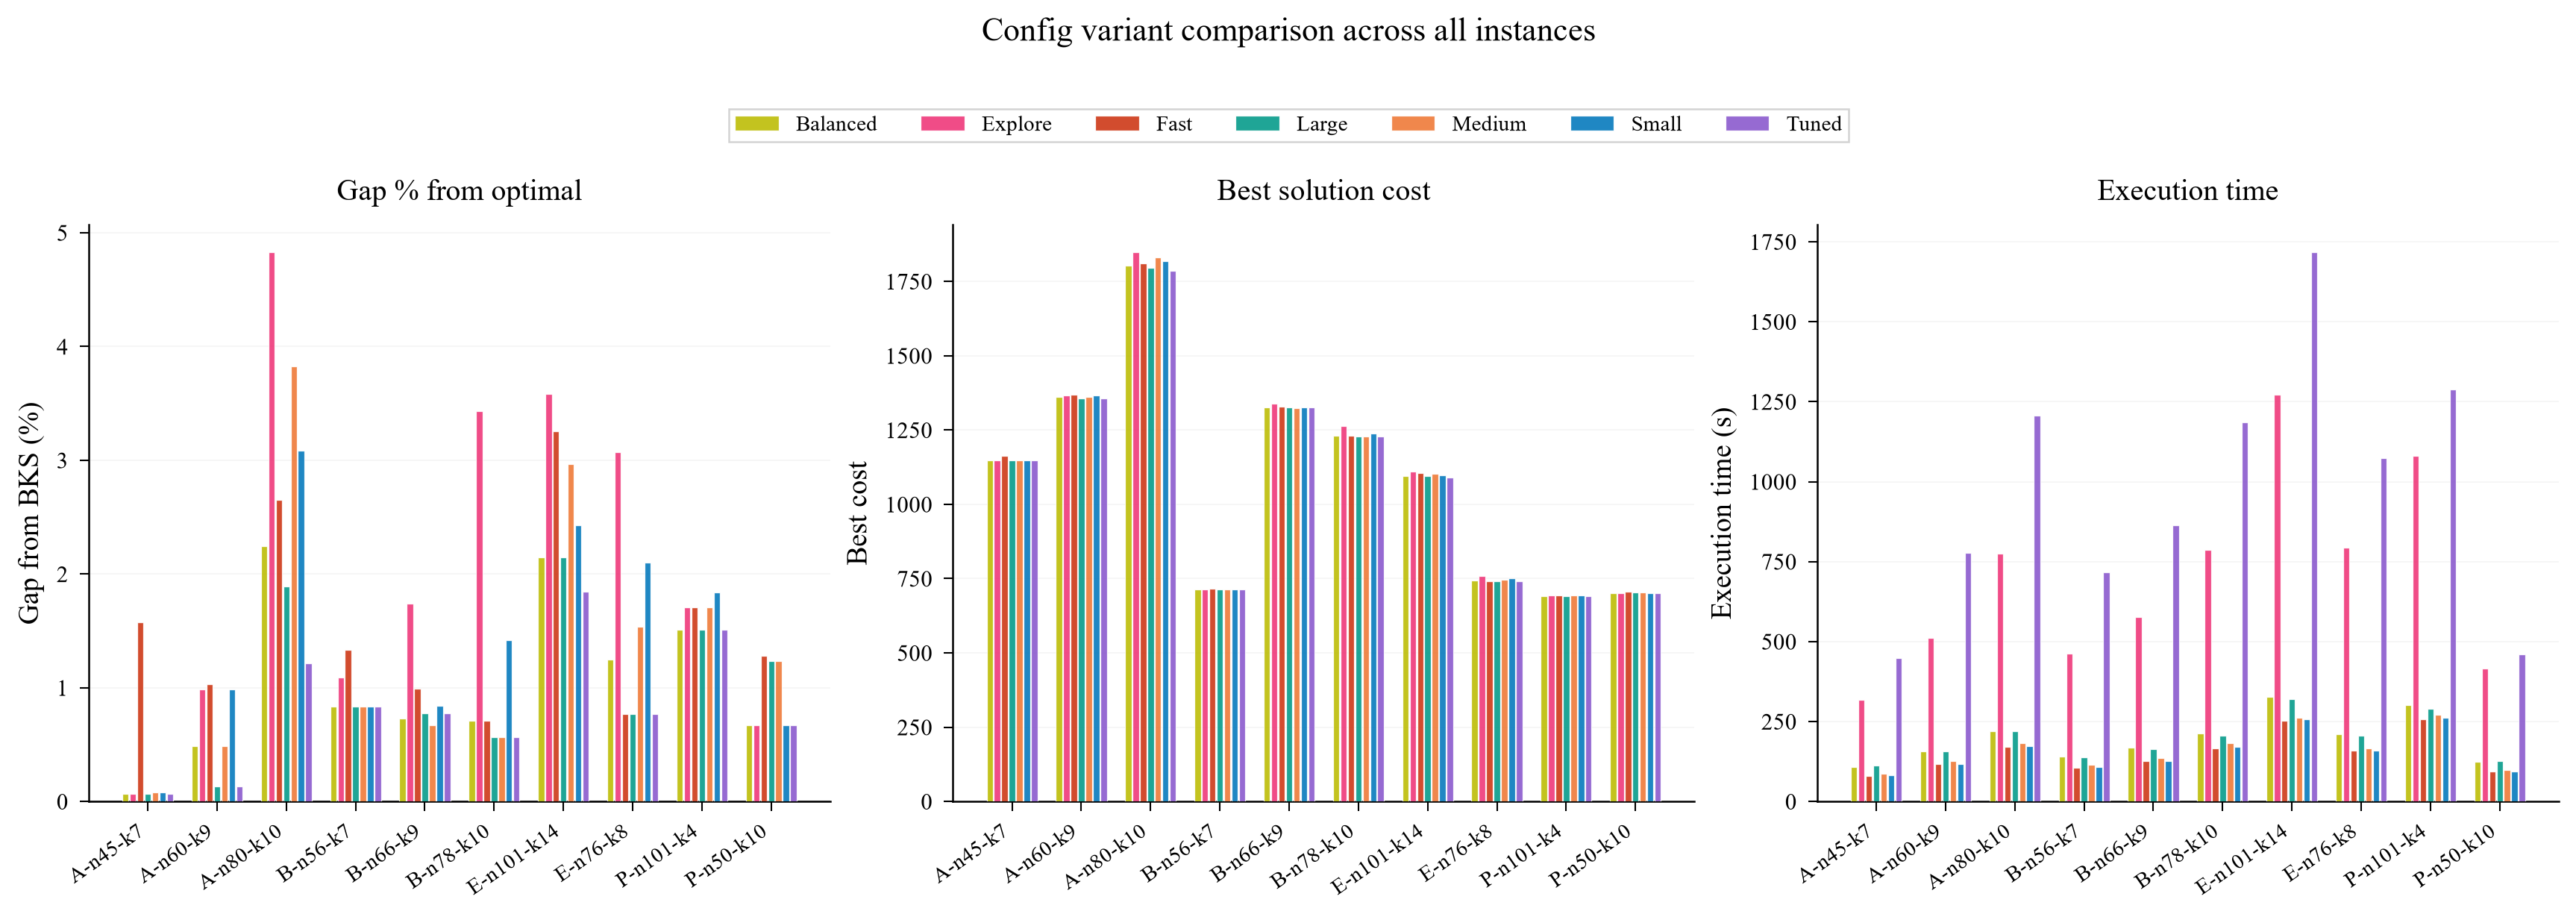
\includegraphics[width=0.95\textwidth]{imgs/summary/summary_config_comparison.png}
    \caption{Confronto visivo tra le quattro varianti di configurazione: gap \%, costo migliore e tempo di esecuzione.}
    \label{fig:config-comparison}
\end{figure}

\subsection{Discussione dei Risultati}

L'analisi dei risultati e del confronto tra configurazioni permette di trarre
diverse osservazioni:

\begin{itemize}
    \item \textbf{Qualità delle soluzioni}: La configurazione Large ($\mu=100$)
    domina quasi tutte le istanze, confermando che una popolazione numerosa
    abbinata a una buona pressione selettiva ($k=4$) ed elitismo ($e=5$)
    offre la migliore esplorazione dello spazio delle soluzioni. Il gap medio
    è inferiore all'1.2\%, con il risultato migliore su A-n45-k7 (0.07\%).

    \item \textbf{Effetto della dimensione della popolazione}: Riducendo $\mu$
    da 100 a 5, il gap medio peggiora progressivamente (Large: $\sim$1.0\%,
    Ultra: $\sim$1.7\%). Il degrado è particolarmente evidente su A-n45-k7
    (da 0.07\% a 1.58\%) e A-n80-k10 (da 1.89\% a 2.65\%). Sorprendentemente,
    su alcune istanze (A-n80-k10, B-n78-k10) la configurazione Ultra supera
    Small e Medium, suggerendo che l'altissimo numero di generazioni compensa
    parzialmente la scarsa diversità.

    \item \textbf{Robustezza}: La deviazione standard è generalmente contenuta
    in tutte le configurazioni, indicando che l'algoritmo è intrinsecamente
    stabile. La configurazione Large mostra la variabilità minore, con
    $\sigma < 1$ su diverse istanze.

    \item \textbf{Velocità di convergenza}: L'ibridazione con ricerca locale
    accelera la convergenza iniziale in tutte le configurazioni. La Large,
    con $\gamma=15$, beneficia di una ricerca locale granulare più ampia
    che contribuisce ai risultati superiori.

    \item \textbf{Trade-off qualità/tempo}: Le configurazioni con popolazione
    minore sono più veloci (meno tempo per generazione) ma richiedono più
    generazioni per convergere. Il tempo totale è dominato dal numero di
    valutazioni FE (fissato a 350.000), quindi tutte le configurazioni
    hanno tempi comparabili.
\end{itemize}

%==================================================
\section{Scelte Progettuali e Originalità}
%==================================================

\subsection{Scelte Chiave}

\begin{enumerate}[label=\textbf{\arabic*.}]
    \item \textbf{Split Algorithm}: L'uso dello split di Prins come decodifica è fondamentale. Invece di codificare esplicitamente le route nel cromosoma, si lascia che la DP trovi la partizione ottimale, riducendo lo spazio di ricerca e garantendo l'ottimalità della decodifica data la permutazione.
    
    \item \textbf{Popolazione iniziale ibrida}: La combinazione di euristiche costruttive (NN, Savings) con permutazioni casuali fornisce un buon punto di partenza senza sacrificare la diversità.
    
    \item \textbf{Set diversificato di operatori LS}: L'inclusione di operatori sia intra-route (2-opt, Or-opt) che inter-route (Relocate, Exchange) permette di migliorare la soluzione a diversi livelli di granularità.
    
    \item \textbf{Probabilità differenziate per mutazione}: Assegnare probabilità diverse agli operatori di mutazione (swap 40\%, insert 30\%, inversion 30\%) riflette la loro diversa efficacia esplorativa.
\end{enumerate}

\subsection{Difficoltà Affrontate}

\begin{itemize}
    \item \textbf{Vincoli di capacità}: Gestire i vincoli di capacità durante il crossover e la mutazione è complesso perché questi operatori lavorano sulla permutazione, non sulle route. Lo split algorithm risolve elegantemente questo problema.
    \item \textbf{Bilanciamento esplorazione-sfruttamento}: Trovare il giusto tasso di ricerca locale ($p_{ls} = 0.1$) è stato cruciale: troppo alto causa convergenza prematura, troppo basso rallenta il miglioramento.
    \item \textbf{Scalabilità}: Su istanze con 101 nodi, lo split $O(n^2)$ e la ricerca locale diventano computazionalmente significativi, richiedendo attenzione all'efficienza implementativa.
\end{itemize}

\subsection{Elementi di Originalità}

\begin{itemize}
    \item \textbf{Architettura client-server con WebSocket}: L'algoritmo è integrato in un'architettura moderna con backend Python (FastAPI) e frontend React, permettendo la visualizzazione in tempo reale dell'evoluzione dell'algoritmo tramite WebSocket.
    \item \textbf{Visualizzazione interattiva}: Il frontend mostra simultaneamente la disposizione geografica delle route, i grafici di convergenza e le statistiche aggregate, offrendo una visione completa del processo di ottimizzazione.
    \item \textbf{Operatori LS compositi}: La sequenza specifica di operatori LS (2-opt $\rightarrow$ Or-opt $\rightarrow$ Relocate $\rightarrow$ Exchange) è progettata per migliorare prima le singole route, poi le interazioni tra route.
\end{itemize}

%==================================================
\section{Conclusioni}
%==================================================

Il progetto ha dimostrato l'efficacia dell'Hybrid Genetic Algorithm per la risoluzione del Capacitated Vehicle Routing Problem. L'approccio ibrido, che combina la potenza esplorativa degli algoritmi genetici con l'efficacia della ricerca locale, produce soluzioni di alta qualità sulle istanze benchmark CVRPLIB.

I punti di forza dell'implementazione includono:
\begin{itemize}
    \item L'uso dello split algorithm per una decodifica ottimale
    \item Un insieme diversificato di operatori genetici e di ricerca locale
    \item Un'architettura software moderna con visualizzazione in tempo reale
    \item Robustezza e consistenza dei risultati tra run diverse
\end{itemize}

Sviluppi futuri potrebbero includere:
\begin{itemize}
    \item L'implementazione di una ricerca locale più aggressiva (Variable Neighborhood Search)
    \item L'uso di tecniche di diversificazione della popolazione (es. crowding, fitness sharing)
    \item L'ottimizzazione automatica dei parametri tramite tecniche di tuning (es. irace)
    \item L'estensione ad altre varianti del VRP (VRPTW, VRPPD)
\end{itemize}

Il codice sorgente del progetto, comprensivo di backend Python, frontend React e relazione \LaTeX, è disponibile nella repository del progetto.

\newpage
%==================================================
\begin{thebibliography}{9}

\bibitem{dantzig1959}
G.B. Dantzig, J.H. Ramser,
\textit{The Truck Dispatching Problem},
Management Science, 6(1):80--91, 1959.

\bibitem{toth2002}
P. Toth, D. Vigo,
\textit{The Vehicle Routing Problem},
SIAM Monographs on Discrete Mathematics and Applications, 2002.

\bibitem{prins2004}
C. Prins,
\textit{A simple and effective evolutionary algorithm for the vehicle routing problem},
Computers \& Operations Research, 31(12):1985--2002, 2004.

\bibitem{vidal2013}
T. Vidal, T.G. Crainic, M. Gendreau, C. Prins,
\textit{Heuristics for multi-attribute vehicle routing problems: A survey and synthesis},
European Journal of Operational Research, 231(1):1--21, 2013.

\bibitem{goldberg1989}
D.E. Goldberg,
\textit{Genetic Algorithms in Search, Optimization, and Machine Learning},
Addison-Wesley, 1989.

\bibitem{cvrplib}
CVRPLib -- Capacitated Vehicle Routing Problem Library,
\url{https://galgos.inf.puc-rio.br/cvrplib/}

\end{thebibliography}

\end{document}
